\chapter{Results, Analysis and Discussion}\label{cha:Results Analysis and Discussion}
This chapter is a combined presentation of collected results, their analysis and a discussion. First section is a presentation of gathered results. 
Second section, divided into three subsections, introduces the evaluation of questions Q1, Q2 and Q3 respectivly. The last section presents the 
conclusions of gathered data and performed analysis. 
\section{Results}
All results presented in this section derived from two data sets. Each data set was collected separetly. First data set is called variant 1 and second is 
called variant 2. Variant 1 contains 2700 and  variant 2 contains 1350 different maze problems, generated by Binary Tree, Aldous-Broder and Recursive-Backtracker
algorithms. Each maze was a separete instance of a class Grid(), execution time of solution was measured in separeted solvers method without interference of
any additionals proceses. For data collecting all visualisation features were disabled and all data were saved during each iteration to the .csv file.
Variants produced  900 and 450 mazes, of randomly applied size. However $9.56\%$ mazes from variant 2 does not have a solution. All data was collected on
MacBook Pro with an Apple M1 microchip, 8GB RAM and 11.6 macOS Big Sur operating system. All the figures used for analysis were made using the Python GUI application Orange v.3.33.First data set is called variant 1.
Each maze must fulfilled following presumptions:\\
$-$ two dimensional, minimum size 5$\times$5, maksimum size 80$\times$80,\\
$-$ staring point coordinates [0,0], goal point [mazeSize.x - 1, mazeSize.y - 1],\\
$-$ weight of each edge equals 1,\\
\textbf{Variant 1 specific presumptions: }\\
$-$ perfect maze,\\
$-$ no directed edges,\\
$-$ each maze is solvable, there is a direct path from starting point to goal point.\\
\textbf{Variant 2 specific presumptions: }\\
$-$ Unperfect maze,\\
$-$ $50\%$ of randomly added links to the a randolmy selected cells in a maze grid,\\
$-$ $3\%$ of south direction added to a randomly selected cells in a maze grid,\\
$-$ mazes do not have to be solvable.\\
\subsection{Results $-$ variant 1}
%------------------------------------AVERAGE PATH LENGHT---------------------------------------------------------
\subsubsection{Average Path Lenght}
Table 5.1 presents the results of mean path lenght for generated mazes in variant 1. Table includes mean values with the standard deviation.
Acoording to Definition 8 on page 9, paths in cyclic mazes may be infinite therefore there is no data presented for vaiant 2.
    \begin{table}[!h]
        \begin{center} 
            \caption{The mean path lenght with standard deviation of Aldous- Broder, Recursive- Backtracker and Binary Tree mazes.} 
        \begin{tabular}{ c c c } 
        \multicolumn{3}{c}{Maze Type} \\
        \hline
        Aldous&Recursive- Backtracker&Binary Tree\\
        \hline
        $103.17\pm 52.91$&$311.79\pm 227.21$&$59.87\pm 25.87$\\
        \hline
         \end{tabular} 
        \end{center}
         \end{table}
%------------------------------------STEPS TO SOLVE---------------------------------------------------------
\subsubsection{Steps to solve}
In Table 5.2 and 5.3  collects mean number of steps needed to solve a maze with standard deviation. Data is splited by the maze type and maze solvers.
\begin{table}[!h]
    \begin{center} 
        \caption{Variant 1: The mean number of steps needed to solve a Aldous- Broder, Recursive- Backtracker and Binary Tree mazes by Astar,
         BFS and Dijkstra solvers.} 
    \begin{tabular}{ c c c c} 
    \multicolumn{4}{c}{Maze Type} \\
    \hline
    &Aldous&Backtracker&Binary\\
    \hline
    Astar&$592.35\pm 556.10$&$972.30\pm 891.90$&$77.34\pm 30.30$\\
    \hline
    BFS&$1170.84\pm 947.40$&$1227.85\pm 1035.50$&$807.18\pm 752.20$\\
    \hline
    Dijkstra&$1773.54\pm 1364.1$&$1802.86\pm 1341.3$&$1546.35\pm 1252.40$\\
    \hline
     \end{tabular} 
    \end{center}
     \end{table}

     \begin{table}[!h]
        \begin{center} 
            \caption{Variant 2: The mean number of steps needed to solve a Aldous- Broder, Recursive- Backtracker and Binary Tree mazes by Astar,
             BFS and Dijkstra solvers.} 
        \begin{tabular}{ c c c c} 
        \multicolumn{5}{c}{Maze Type} \\
        \hline
        Solver&Aggregate&Aldous-Broder&Recursive-Backtracker&Binary Tree\\
        \hline
        Astar&$154.55\pm 67.60$&$168.14\pm 76.30$&$94.99\pm 45.20$\\
        \hline
        BFS&$990.12\pm 899.10$&$986.93\pm 923.80$&$654.73\pm 721.19$\\
        \hline
        Dijkstra&$1728.08\pm 1361.60$&$1705.73\pm 1386.3$&$1702.16\pm 1318.80$\\
        \hline
         \end{tabular} 
        \end{center}
         \end{table}
    %------------------------------------SOLUTION TIME---------------------------------------------------------
\subsubsection{Solution Time}
Figure 5.1, Table 5.4 and Table 5.5 presents an overview of the measured mean solution time with standard deviation. 
\begin{figure}[!h]
    \centering
    \begin{subfigure}[b]{0.48\textwidth}
        \centering
        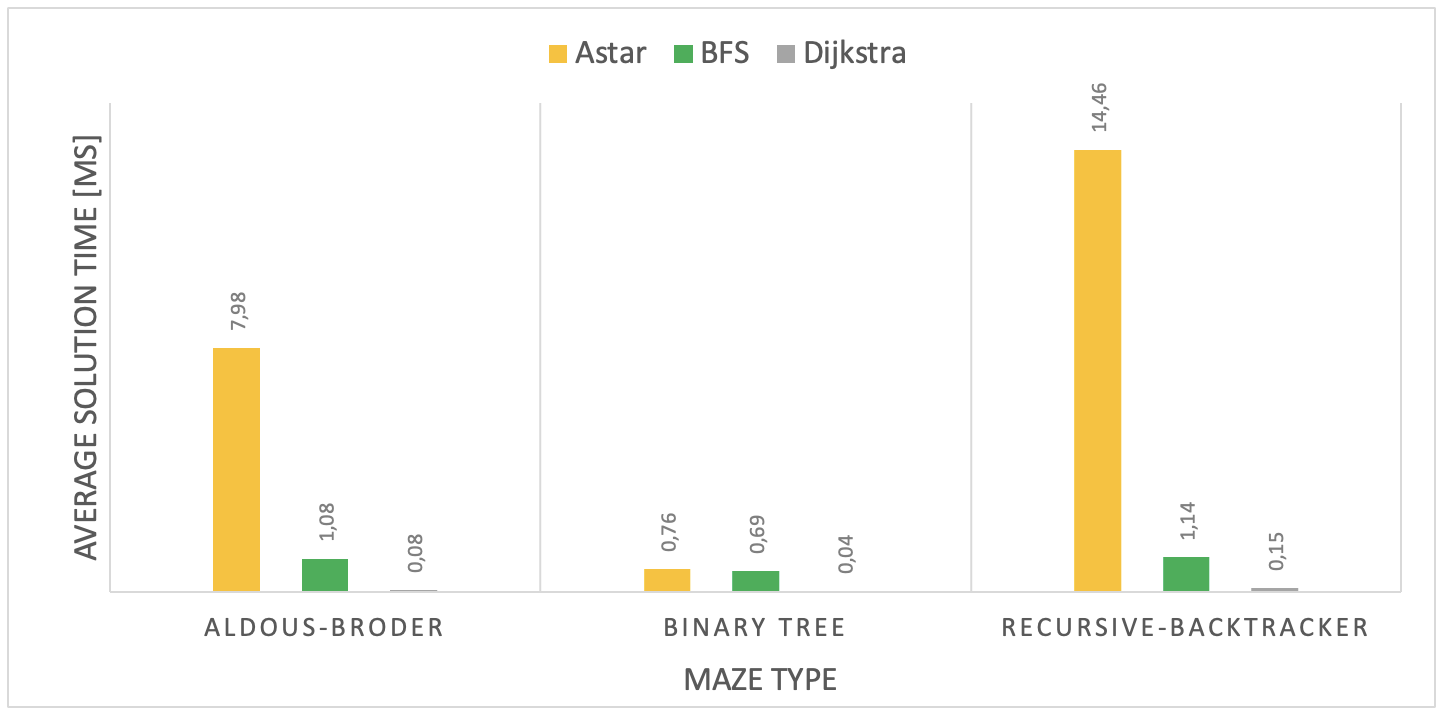
\includegraphics[width=\textwidth]{averagetime_variant1.png}
        \caption{}
    \end{subfigure}
    \begin{subfigure}[b]{0.48\textwidth}  
        \centering 
        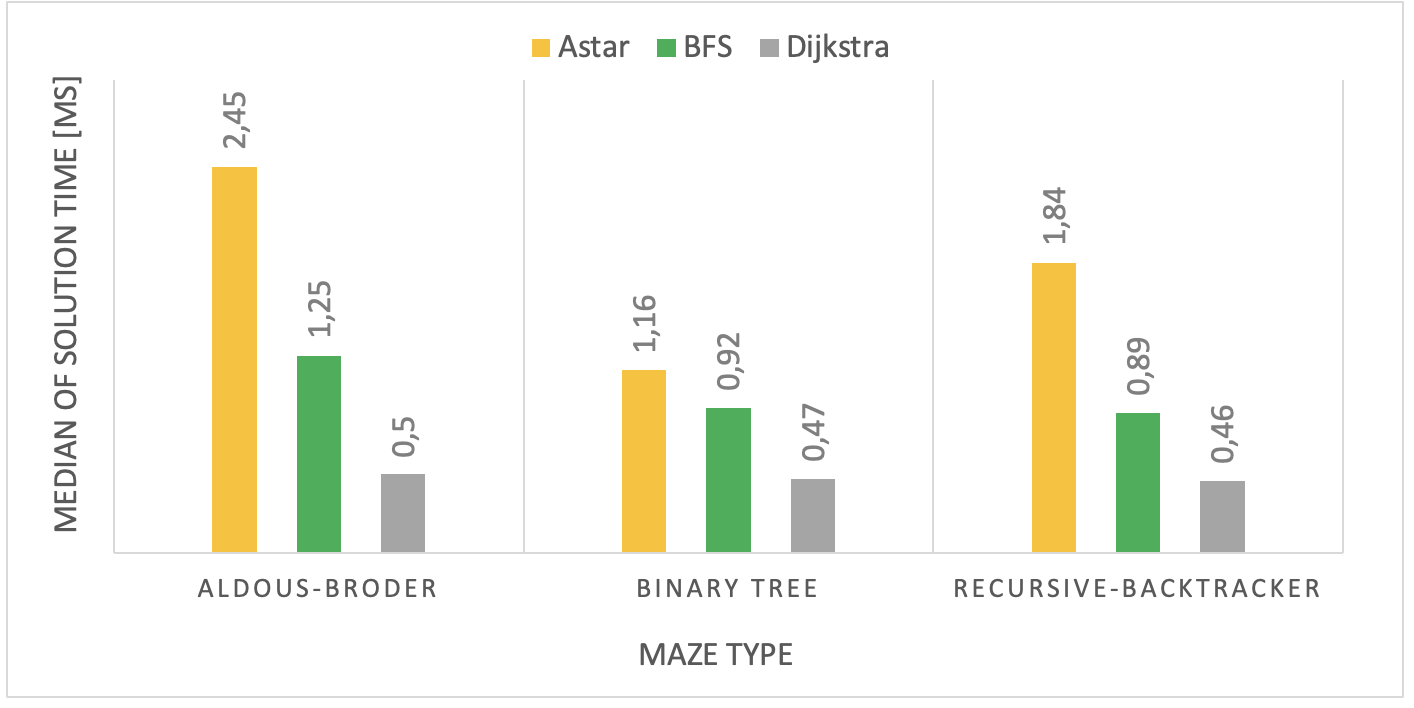
\includegraphics[width=\textwidth]{averagetime_variant2.png}
        \caption{}
    \end{subfigure}
    \caption[]{(a) Variant 1: Solution time for different types of maze showing the maze size versus dijkstra solution time. (b) as for (a) but (b) is 
    Variant 2.}
\end{figure}
\begin{table}[!h]
    \begin{center} 
        \caption{Variant 1: Mean Solution time for different maze solvers of different maze generators.} 
    \begin{tabular}{ c c c c} 
    \multicolumn{4}{c}{Maze Type} \\
    \hline
    &Aldous&Backtracker&Binary\\
    \hline
    Astar&$20.74\pm 40.01$&$47.10\pm 83.53 $&$1.33\pm 1.23$\\
    \hline
    BFS&$1.29\pm 1.05$&$1.38\pm 1.18$&$0.92\pm 1.13$\\
    \hline
    Dijkstra&$0.11\pm 0.097$&$0.20\pm 0.24$&$0.08\pm 0.086$\\  
    \hline
     \end{tabular} 
    \end{center}
     \end{table}
     \begin{table}[!h]
        \begin{center} 
            \caption{Variant 2: Mean solution time for different maze solvers of different maze generators.} 
        \begin{tabular}{ c c c c c} 
        \multicolumn{5}{c}{Maze Type} \\
        \hline
        &Aggregate&Aldous&Backtracker&Binary\\
        \hline
        Astar&Mean&$1.432\pm 1.340$&$2.138\pm 2.041$&$1.666\pm 1.408$\\
        \hline
        BFS&Mean&$0.514\pm 0.544$&$0.759\pm 0.769$&$0.893\pm 0.831$\\
        \hline
        Dijkstra&Mean&$0.415\pm 0.366$&$0.569\pm 0.540$&$0.973\pm 0.781$\\  
        \hline
         \end{tabular} 
        \end{center}
         \end{table}
      %------------------------------------MCCLENDON'S--------------------------------------------------------
\newpage
      \subsubsection{McClendon's Complexity}
In figure 5.2a and a 5.3a a scatter plots of Maze Size versus McClendon's Complexity are presented. Different colours were applied to different solvers.
In Figure 5.2b and 5.3b a box plot of McClendon's Complexity distributions are showing mean complexity with standard deviation and maximal and minimal values is presented.
    \begin{figure}[!h]
        \centering
        \begin{subfigure}[!h]{0.4\textwidth}
           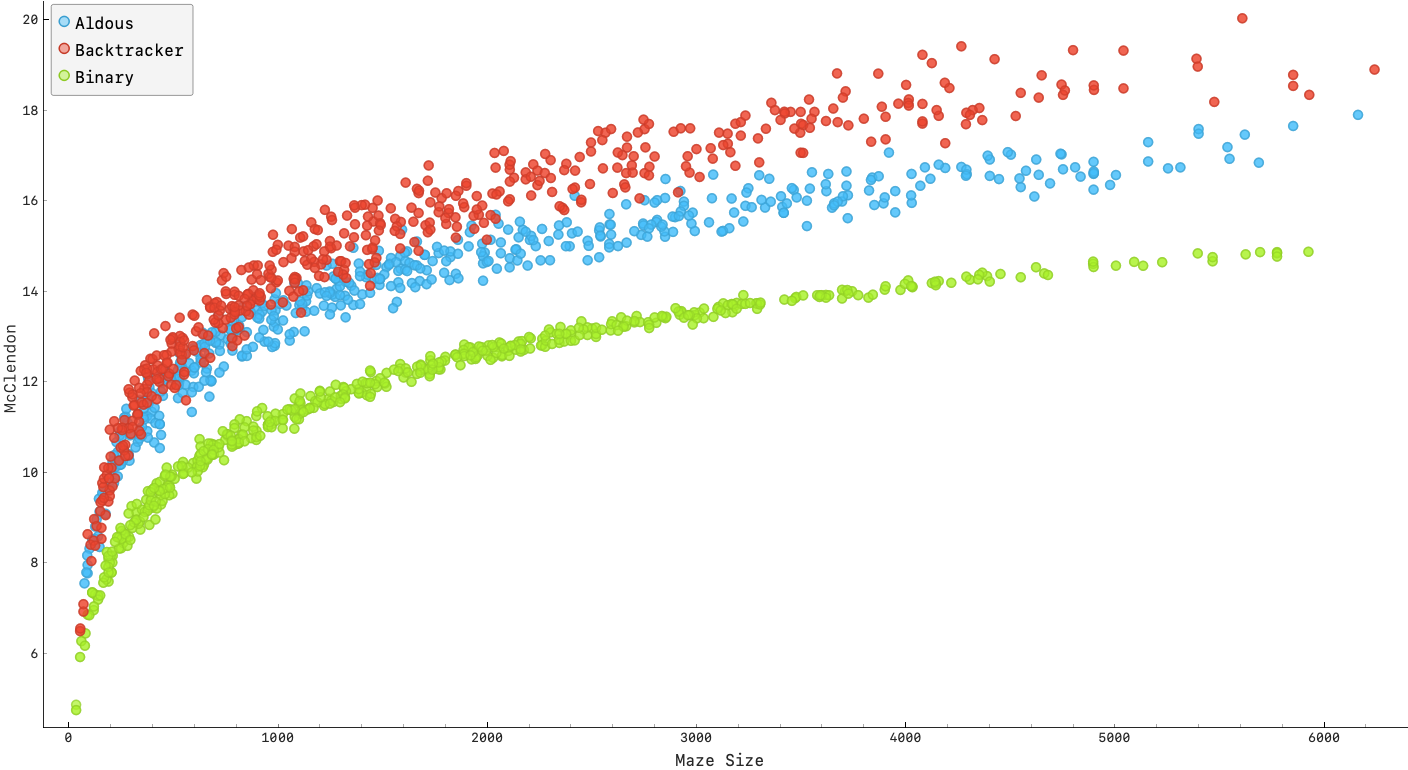
\includegraphics[scale = 0.15]{McClendonVsSize_variant1.png}
           \caption{}
        \end{subfigure}
        
        \begin{subfigure}[!h]{0.5\textwidth}
           \includegraphics[width=1\linewidth]{McClendonANOVA_variant1.png}
           \caption{}
        \end{subfigure}
        \caption{Variant 1: (a) a scatter plot of Maze Size versus McClendon's Complexity with applied colour to different classes of maze solvers.
         (b) a box plot of McClendon Complexity distribution, showing mean with standard deviation for three maze generators.}
        \end{figure}%
        \begin{figure}[!h]
            \centering
            \begin{subfigure}[!h]{0.4\textwidth}
               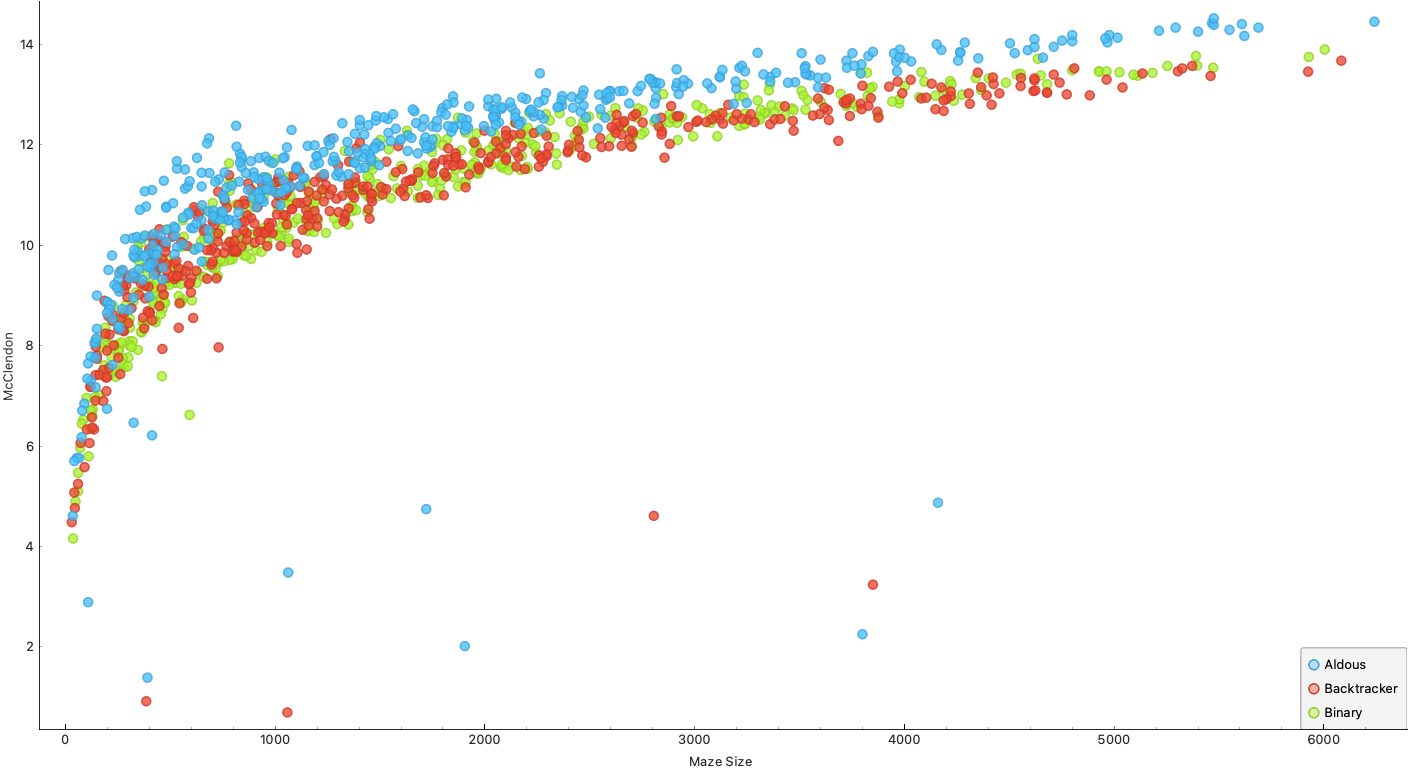
\includegraphics[scale =0.15]{McClendonvsSize_variant2.png}
               \caption{}
            \end{subfigure}
            \begin{subfigure}[!h]{0.5\textwidth}
               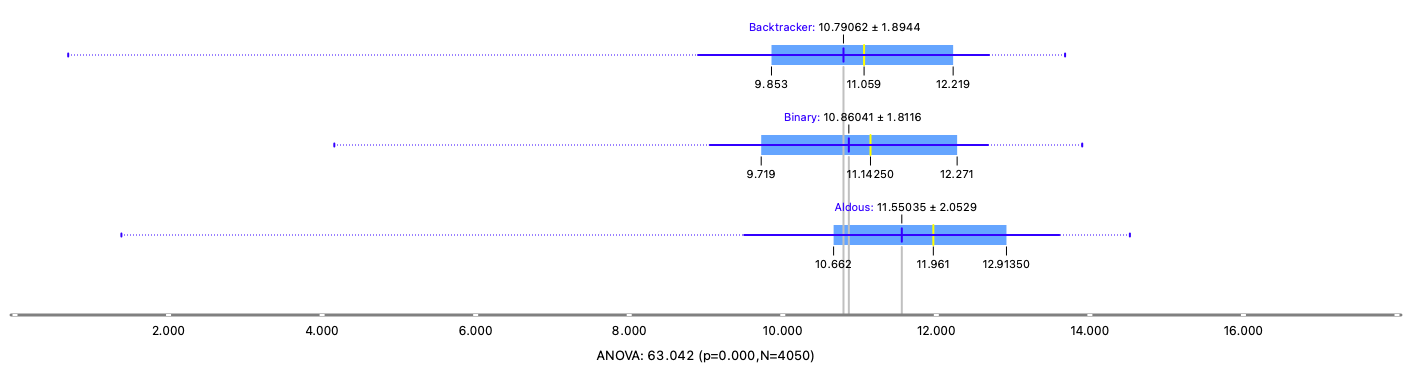
\includegraphics[width=1\linewidth]{McClendon_variant2.png}
               \caption{}
            \end{subfigure}
            \caption{Variant 2: (a) a scatter plot of Maze Size versus McClendon's Complexity with applied colour to different classes of maze solvers.
             (b) a box plot of McClendon Complexity distribution, showing mean with standard deviation values for three maze generators.}
            \end{figure}%
 %------------------------------------SHANONS ENTROPY---------------------------------------------------------
\newpage
 \subsubsection{Shanonn's Entropy}
In figure 5.4a and 5.5a a scatter plots of Maze Size versus Shanonn's Entropy are presented. Different colours were applied to different solvers. In Figure 5.4b
and 5.5b a box plot of Shanonn's Entropy are presented. Showing mean entropy with a standard deviation values.
    \begin{figure}[!h]
        \centering
        \begin{subfigure}[!h]{0.4\textwidth}
           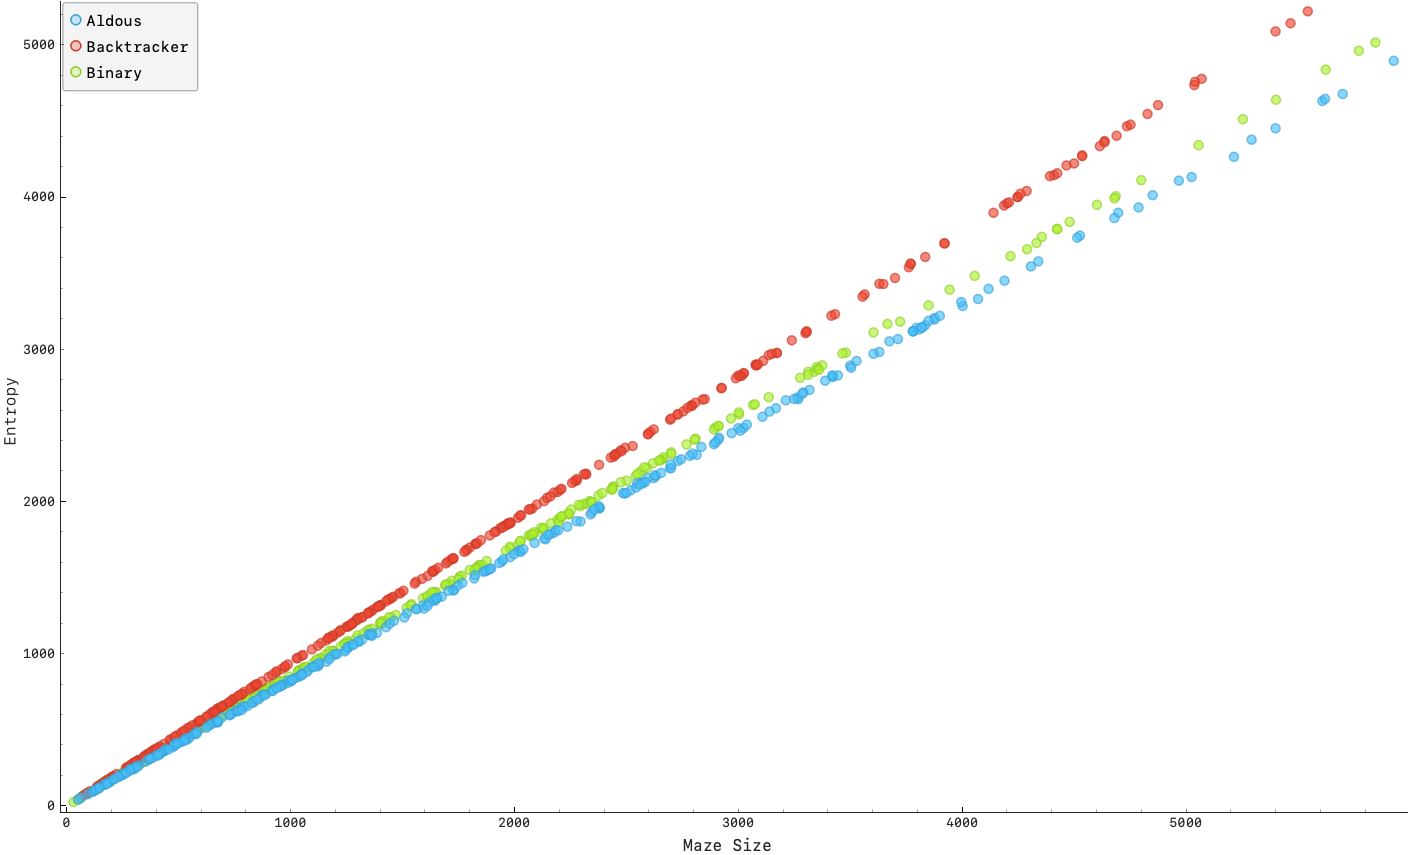
\includegraphics[scale = 0.15]{EntropyVsSize_variant1.png}
           \caption{}
        \end{subfigure}
        \begin{subfigure}[!h]{0.6\textwidth}
           \includegraphics[width=1\linewidth]{EntropyANOVA_variant1.png}
           \caption{}
        \end{subfigure}
        \caption{(a) Variant 1: a scatter plot of Maze Size versus Shannon's Entropy with applied colour to different classes of maze solvers.
        (b) a box blot of Shannon's Entropy distribution for different maze generator showing mean with standard deviation values}
        \end{figure}

        \begin{figure}[!h]
            \centering
            \begin{subfigure}{0.4\textwidth}
               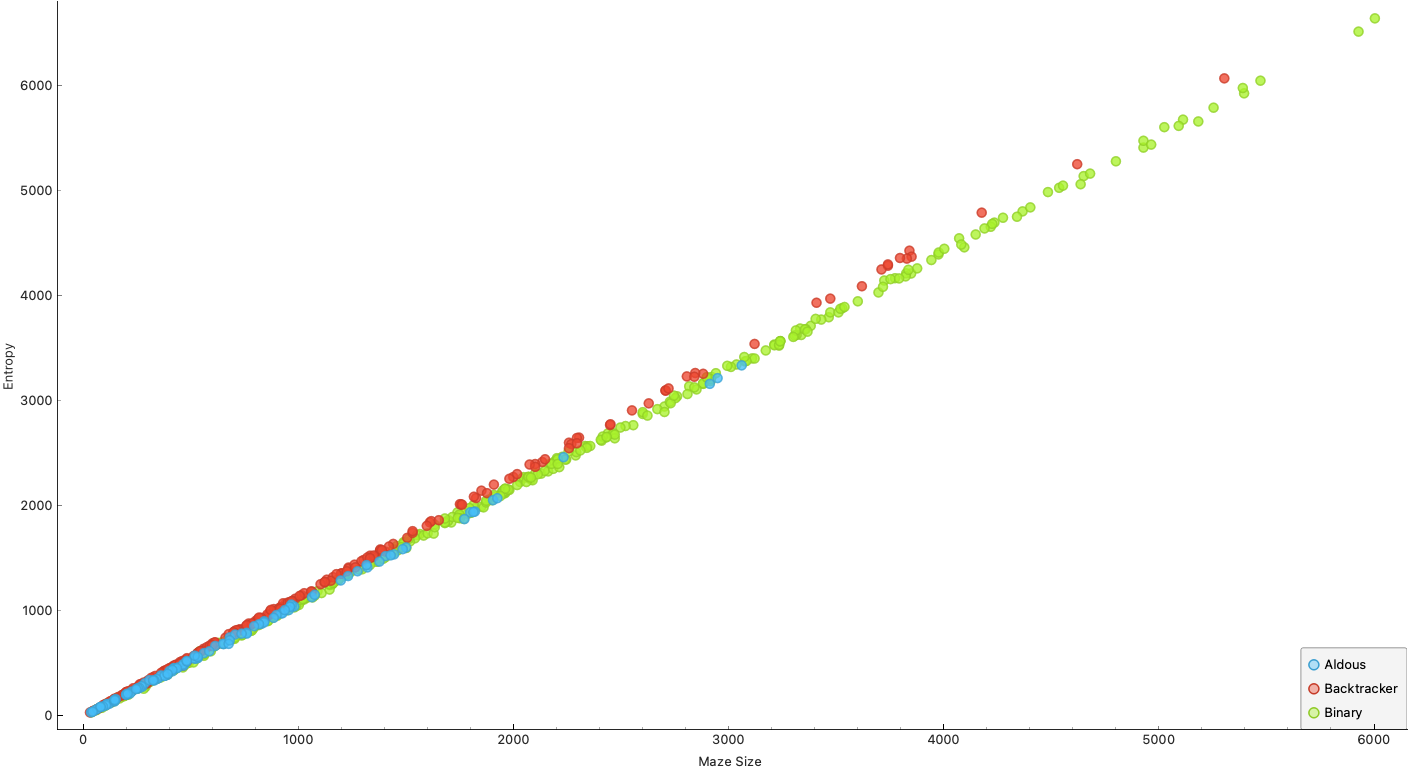
\includegraphics[scale = 0.15]{entropyvssize_variant2.png}
               \caption{}
            \end{subfigure}
            \begin{subfigure}{0.5\textwidth}
               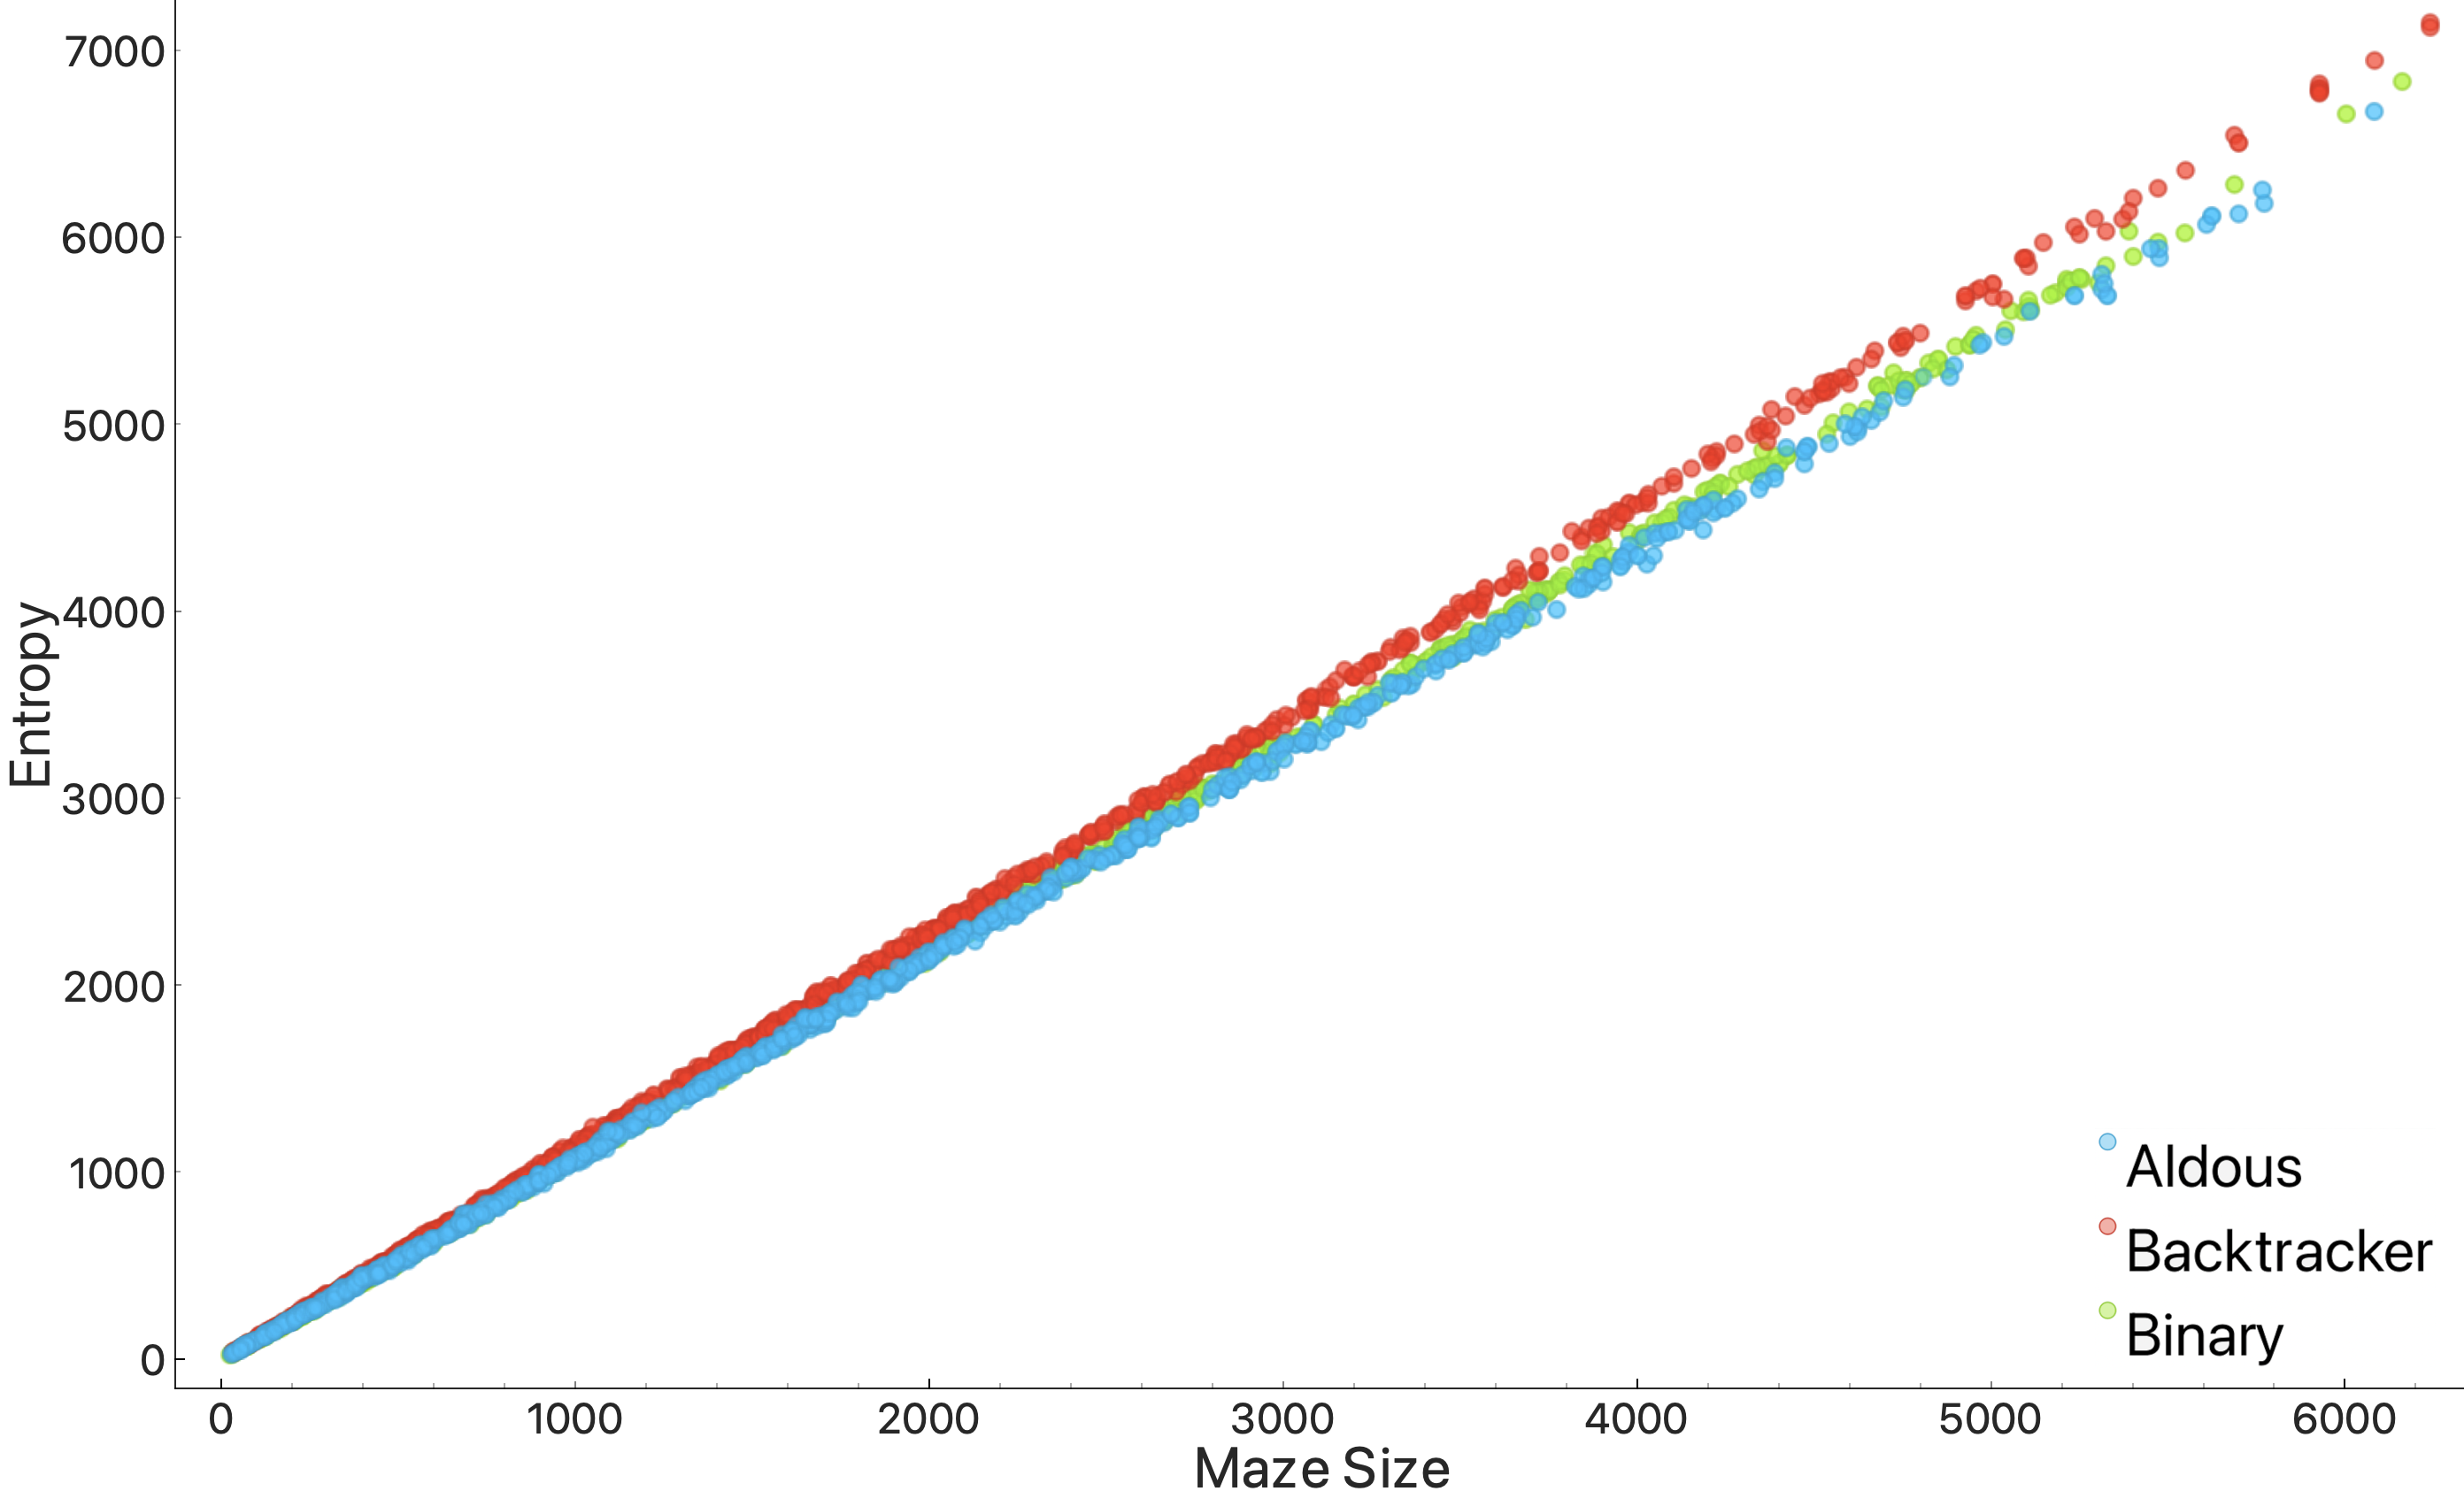
\includegraphics[width=1\linewidth]{entropy_variant2.png}
               \caption{}
            \end{subfigure}
            \caption{(a) Variant 2:  a scatter plot of Maze Size versus Shannon's Entropy with applied colour to different classes of maze solvers.
            (b) a box blot of Shannon's Entropy distribution for different maze generator showing mean with standard deviation values}
            \end{figure}
\newpage
%------------------------------------DEGREE DISTRIBUTION--------------------------------------
\subsubsection{Degree Distribution}  
In Table 5.6 and 5.7 statistical information about degree distribution for different type of mazes is presented on box plot for each vertex degree type.
Figures 5.6 and 5.7 presents a scatter plot of a deadend ratio versus a cross ratio, different colours differentciate maze generators.

\begin{table}[!h]
    \begin{center} 
        \caption{Variant 1: Degree distribution for three maze generators: Binary Tree, Aldous-Broder and Recursive- Backtracker} 
    \begin{tabular}{ c c c c c} 
    \multicolumn{5}{c}{Maze Type} \\
    \hline
    &Aggregate&Aldous&Backtracker&Binary\\
    \hline
Deadend Ratio&Mean&$0.291\pm 0.011$&$0.1021\pm 0.0065$&$0.2512\pm 0.0097$\\    
    \hline
Fork Ratio&Mean&$0.455\pm 0.020$&$0.800\pm 0.012$&$0.501\pm 0.019$\\
    \hline
Intersection Ratio&Mean&$0.220\pm 0.011$&$0.096\pm 0.011$&$0.248\pm 0.010$\\    
    \hline
Cross Ratio&Mean&$0.034\pm 0.006$&$0.001\pm 0.001$&$0\pm 0$\\    
    \hline   
     \end{tabular} 
    \end{center}
     \end{table}

     \begin{table}[!h]
        \begin{center} 
            \caption{Variant 2: Degree distribution for three maze generators: Binary Tree, Aldous-Broder and Recursive- Backtracker} 
        \begin{tabular}{ c c c c c} 
        \multicolumn{5}{c}{Maze Type} \\
        \hline
        &Aggregate&Aldous&Backtracker&Binary\\
        \hline
    Deadend Ratio&Mean&$0.169\pm 0.025$&$0.067\pm 0.013$&$0.146\pm 0.017$\\    
        \hline
    Fork Ratio&Mean&$0.427\pm 0.034$&$0.575\pm 0.026$&$0.436\pm 0.019$\\ 
        \hline
    Intersection Ratio&Mean&$0.328\pm 0.025$&$0.325\pm 0.024$&$0.361\pm 0.021$\\   
        \hline
    Cross Ratio&Mean&$0.077\pm 0.021$&$0.034\pm 0.010$&$0.057\pm 0.010$\\   
        \hline   
         \end{tabular} 
        \end{center}
         \end{table}
         \begin{figure}[!h]
            \centering
            \begin{subfigure}[!h]{0.47\textwidth}
                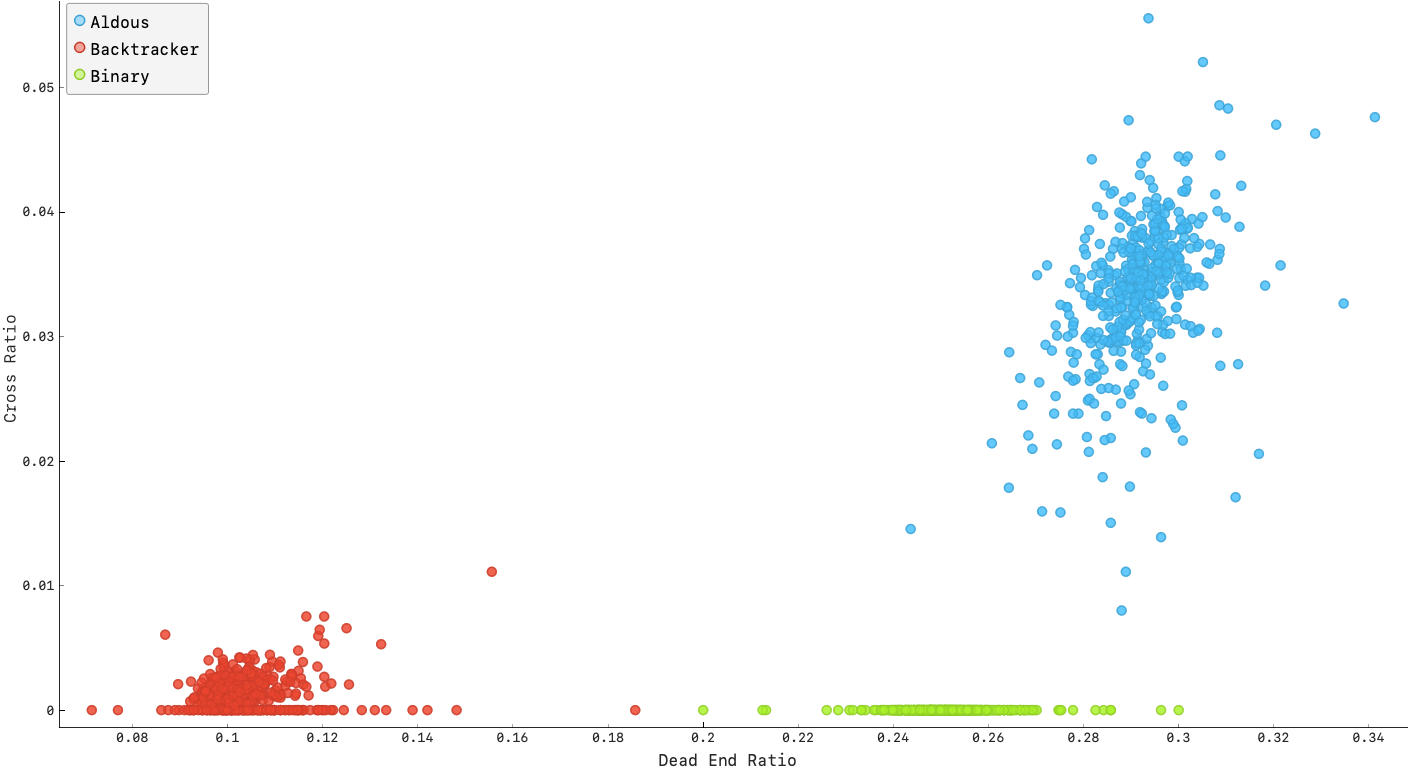
\includegraphics[scale = 0.17]{CrossVsDeadEnd_variant1.png}
               \caption{}
            \end{subfigure}
            \begin{subfigure}[!h]{0.47\textwidth}
                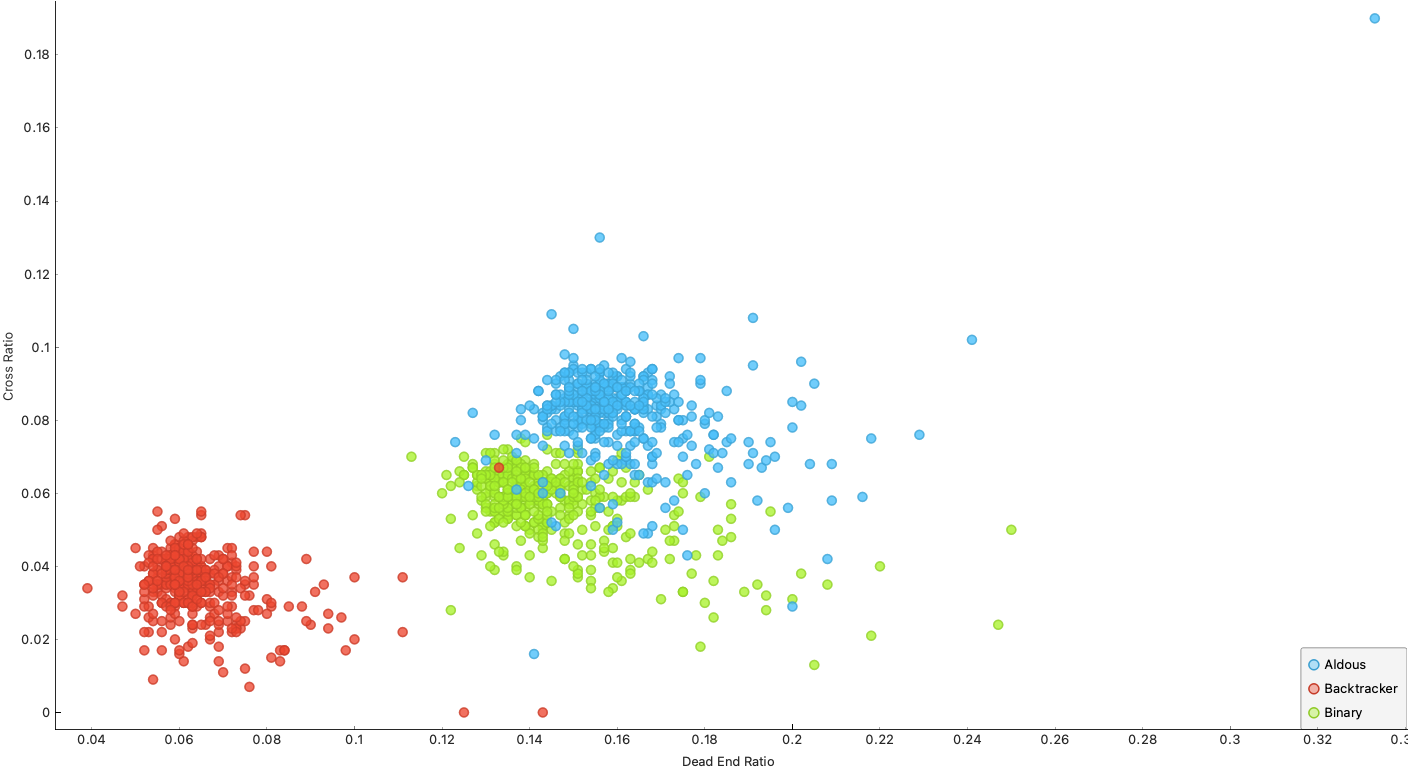
\includegraphics[scale = 0.17]{CrossVsDeadEnd_variant2.png}
               \caption{}
            \end{subfigure}
            \caption{Variant 1: A scatter plot of deadent ratio versus cross ratio, different coulours distinguish different maze generators.}
            \end{figure}
\newpage
\section{Practical analysis of maze generators and maze solvers}
In this section, all algorithms described in Chapter 4 are assessed in terms of their runtime and parameters of generated solutions. Three algorithms described
in Chapter 4 were evaluated: Dijkstra, $A^*$ and BFS, each algorithm was tested in the same way. The runtime measurement program worked as follows,
the program generated a random-sized maze using one of the three algorithms: Binary Tree, Recursive Backtracker, or Aldous-Broder. Then each solving
algorithm one by one was applied to solve the same problem. Mazes were generated with randomly assigned size ranging from $5 \times 5$ to $80 \times 80$.
The main assumption was to create a rectangular maze with the source cell $p$ at the left top corner, and goal cell $q$ at the right bottom corner of the maze grid. 
All solvers could only use the NSWE moves described in Chapter 4. Maze problems usually have quick access to basic heuristic functions because of
a graph implemented as a grid. Because of the assumption that only the NSWE moves are allowed the heuristic method $h(v)$ applied in $A^*$ was the
Manhattan Distance.
The purpose is to compare both the maze generators and the solvers and build a framework which could classify which algorithms comply best with each other.
Although the runtime of both, the generating and solving algorithms were measured, it was not the purpose of this work to minimize it. Therefore, the algorithms
were implemented in JavaScript. It's beyond discussion that the implementation in a more low-level language would be more efficient, and could lead to building
and solving bigger mazes. However, the choice of using Java Script for algorithm implementation was dictated by the eagerness of building a web application
depending on and harnessing the results of this work. 
The reprezentative set of solved mazes is presented in Figure 5.1.%tutaj dołozyć inne rodzaje mazów
\begin{figure}[!h]
	\centering
	\begin{subfigure}{.33\textwidth}
	  \centering
	  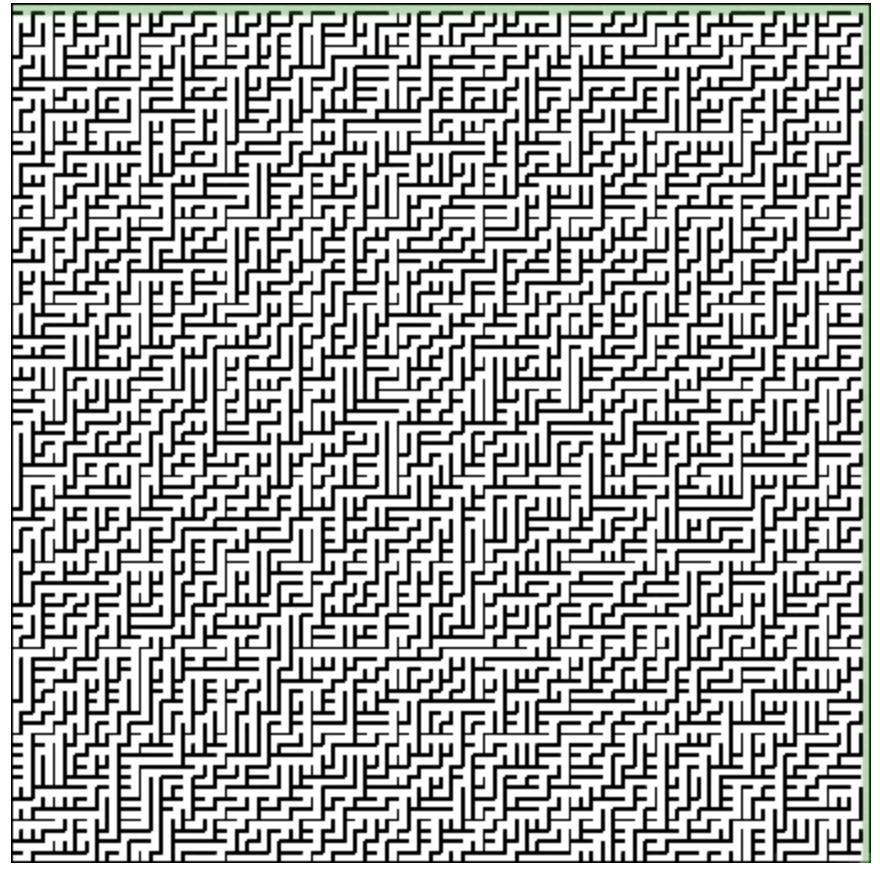
\includegraphics[width=1\linewidth]{perfectBinary.png}
	  \caption{}
	  \label{fig:sub1}
	\end{subfigure}
	\begin{subfigure}{.33\textwidth}
	  \centering
	  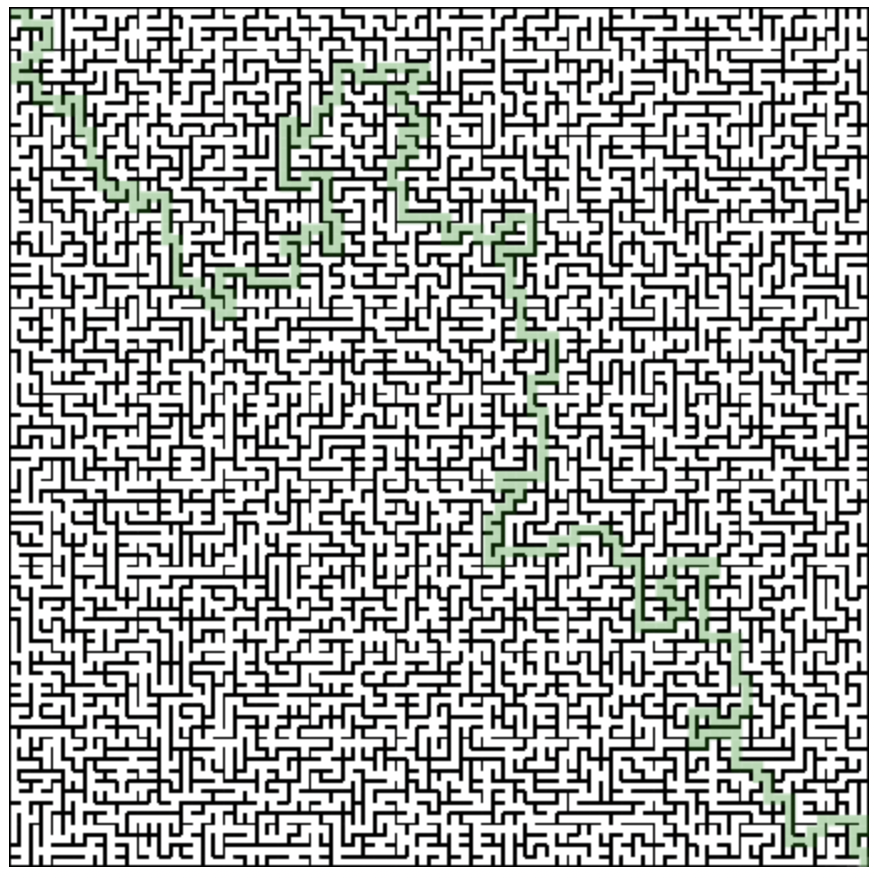
\includegraphics[width=1\linewidth]{perfectAldous.png}
	  \caption{}
	  \label{fig:sub2}
	\end{subfigure}
    \begin{subfigure}{.33\textwidth}
        \centering
        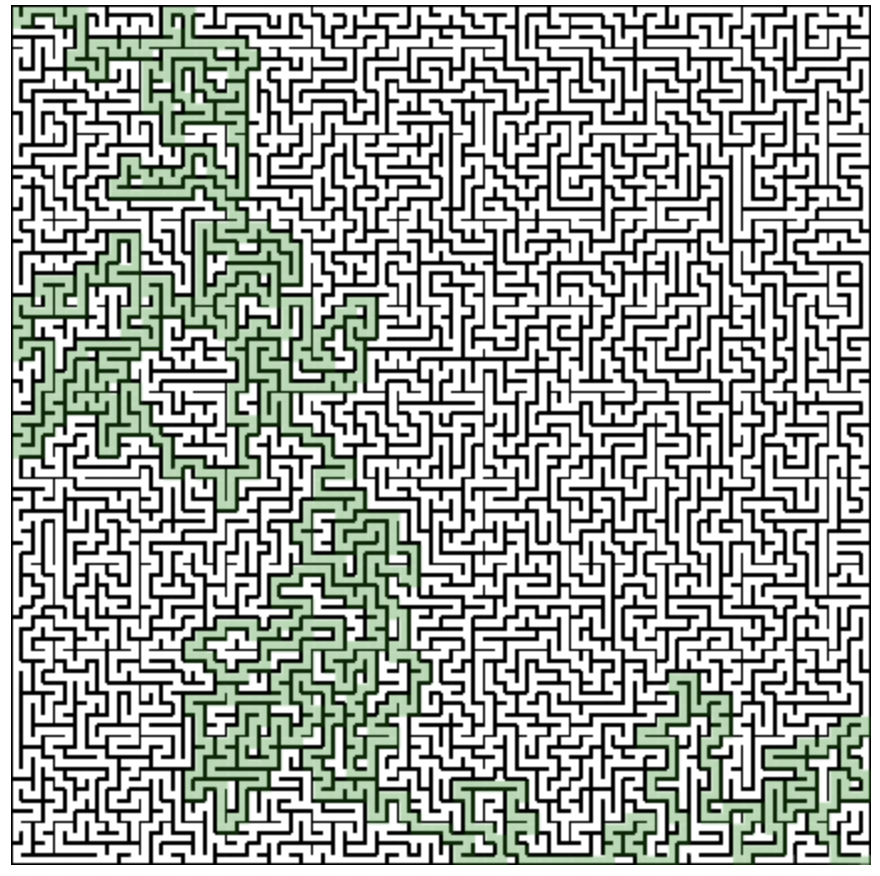
\includegraphics[width=1\linewidth]{perfectRecursive.png}
        \caption{}
        \label{fig:sub2}
      \end{subfigure}
	\caption{Examples of different, perfect,  80 $\times$ 80 mazes with applied Dijkstra solution. In subfigure (a) there is a Binary Tree maze, \\Source: developed by the author}
	\label{fig:test}
	\end{figure}
\subsection{Path and time comparison for different maze solvers}Q1
The algorithm which generates mazes with the longest mean path is Recursive- Backtracker, which is $311.79\pm 227.21$. The shortest mean paths are generated by
Binary Tree algorithm, which is $59.87\pm 87$. A significant value of the mean path length might indicates a higher number of longer paths in the maze. That 
may results in a longer solution time due to the greater number of long side paths, i.e. paths that are not a solution. This is also confirmed by the results of
the measured time and number of steps, which are also the biggest for Recursive-Backtracker, and the smallest for Binary Tree for every solver as showed in 
Table 1.2, Table 1.4 and Figure 5.1a. What is noticable for this data set is a very big standard deviation, which might be caused by big maze size range.
The results for Aldous-Broder mazes fall  between Recursive- Backtracker and Binary as well as for solution time, mean path lengh and steps needed to solve.

Solution Time for Dijkstra is the shortest regardless the size and maze type. Mean time for dijkstra does not exceed 0.2ms for each type of maze.
The longest solution time was measured for astar solver for which the worst case is 47.1 ms for solving a recursive-backtracker maze.
However, the astar solution time varies a lot depending on the maze generator which is visible oin Figure 5.1a and in Table 1.4
 

Mean solution time for asta

 
\subsection{Analysis of parameters affecting maze complexity}Q2
\subsection{Parametrizing the maze problem for choosing the best solver}Q3
\section{Conclusion}
